\documentclass[preprint, 3p,
authoryear]{elsarticle} %review=doublespace preprint=single 5p=2 column
%%% Begin My package additions %%%%%%%%%%%%%%%%%%%

\usepackage[hyphens]{url}

  \journal{GEOG 712 Reproducible Research Workflow with GitHub and
R} % Sets Journal name

\usepackage{graphicx}
%%%%%%%%%%%%%%%% end my additions to header

\usepackage[T1]{fontenc}
\usepackage{lmodern}
\usepackage{amssymb,amsmath}
% TODO: Currently lineno needs to be loaded after amsmath because of conflict
% https://github.com/latex-lineno/lineno/issues/5
\usepackage{lineno} % add
\usepackage{ifxetex,ifluatex}
\usepackage{fixltx2e} % provides \textsubscript
% use upquote if available, for straight quotes in verbatim environments
\IfFileExists{upquote.sty}{\usepackage{upquote}}{}
\ifnum 0\ifxetex 1\fi\ifluatex 1\fi=0 % if pdftex
  \usepackage[utf8]{inputenc}
\else % if luatex or xelatex
  \usepackage{fontspec}
  \ifxetex
    \usepackage{xltxtra,xunicode}
  \fi
  \defaultfontfeatures{Mapping=tex-text,Scale=MatchLowercase}
  \newcommand{\euro}{€}
\fi
% use microtype if available
\IfFileExists{microtype.sty}{\usepackage{microtype}}{}
\usepackage[]{natbib}
\bibliographystyle{elsarticle-harv}

\usepackage{graphicx}
\ifxetex
  \usepackage[setpagesize=false, % page size defined by xetex
              unicode=false, % unicode breaks when used with xetex
              xetex]{hyperref}
\else
  \usepackage[unicode=true]{hyperref}
\fi
\hypersetup{breaklinks=true,
            bookmarks=true,
            pdfauthor={},
            pdftitle={Food Deserts or Food Oases? Predicting Grocery Store Locations in Hamilton, Ontario},
            colorlinks=false,
            urlcolor=blue,
            linkcolor=magenta,
            pdfborder={0 0 0}}

\setcounter{secnumdepth}{5}
% Pandoc toggle for numbering sections (defaults to be off)


% tightlist command for lists without linebreak
\providecommand{\tightlist}{%
  \setlength{\itemsep}{0pt}\setlength{\parskip}{0pt}}




\usepackage{tabularx}
\usepackage{float}
\floatplacement{figure}{H}




\begin{document}


\begin{frontmatter}

  \title{Food Deserts or Food Oases? Predicting Grocery Store Locations
in Hamilton, Ontario}
    \author[sees]{Zehui Yin%
  \corref{cor1}%
  }
   \ead{yinz39@mcmaster.ca} 
      \affiliation[sees]{
    organization={School of Earth, Environment \& Society, McMaster
University},addressline={1280 Main Street
West},city={Hamilton},postcode={L8S
4K1},state={Ontario},country={Canada},}
    \cortext[cor1]{Corresponding author}
  
  \begin{abstract}
  This is the abstract.

  It consists of two paragraphs.
  \end{abstract}
    \begin{keyword}
    Grocery Store \sep 
    Hamilton
  \end{keyword}
  
 \end{frontmatter}

\section{Introduction}\label{introduction}

Nice introduction goes here\ldots{}

\section{Data and Methods}\label{data-and-methods}

\subsection{Study Area}\label{study-area}

My study area is Hamilton, Ontario. Figure \ref{fig::study_area} below
shows the study area.

\begin{figure}
\centering
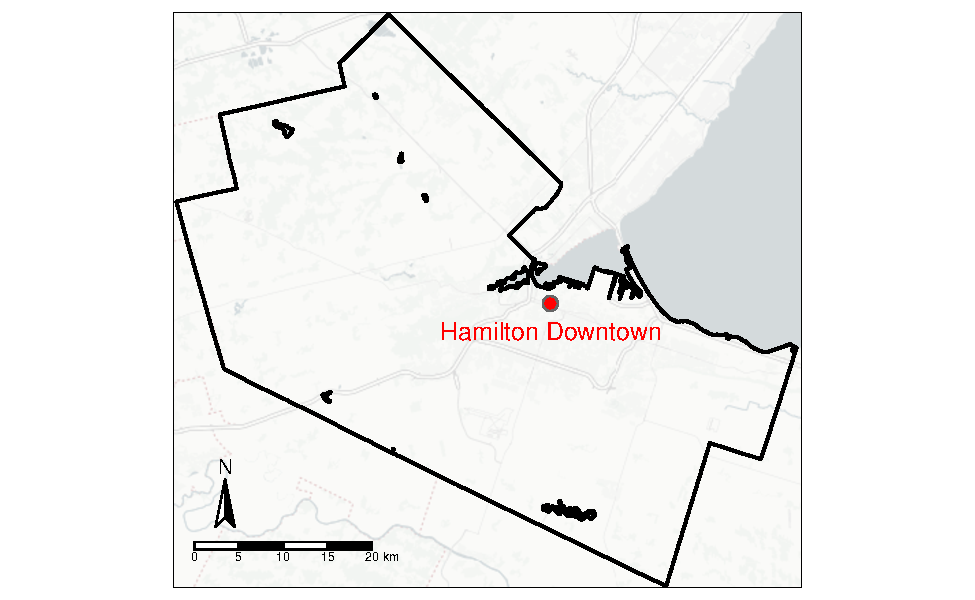
\includegraphics{grocery_store_hamilton_files/figure-latex/unnamed-chunk-4-1.pdf}
\caption{\label{fig::study_area}Study Area: Hamilton, Ontario}
\end{figure}

\subsection{Data Sources}\label{data-sources}

My data used in this project are shown in Table \ref{tab:data_source}
below.

\begin{table}[h]
\centering
\begin{footnotesize}
\begin{tabularx}{\textwidth}{XllXl}
\hline
Name                                           & Source             & URL                                             & Accessed Date \\
\hline
Grocery Stores in Hamilton                     & OpenStreetMap      & \url{https://overpass-turbo.eu/index.html}      & 2024-10-04    \\
HSR Fall 2024 GTFS Static                      & Hamilton Open Data & \url{https://opendata.hamilton.ca/GTFS-Static/} & 2024-10-04    \\
Dissemination Area and Census Data in Hamilton & Statistics Canada  & \url{https://censusmapper.ca/api}               & 2024-11-16    \\
\hline
\end{tabularx}
\caption{\label{tab:data_source}Data Sources}
\end{footnotesize}
\end{table}

\subsection{Methodology}\label{methodology}

\section{Results}\label{results}

\subsection{Descriptive Statistics}\label{descriptive-statistics}

\begin{figure}
\centering
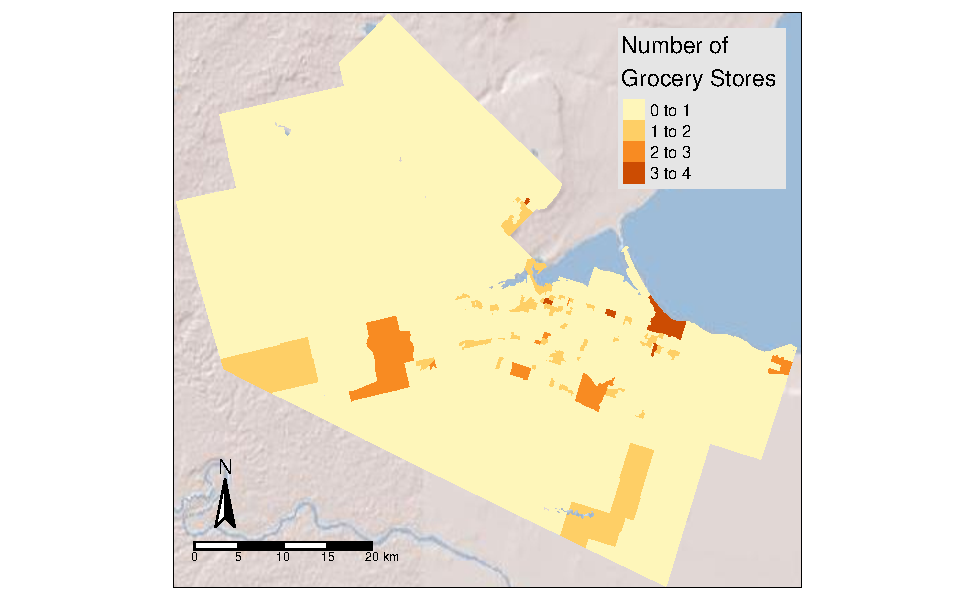
\includegraphics{grocery_store_hamilton_files/figure-latex/unnamed-chunk-9-1.pdf}
\caption{\label{fig::grocery_DA}Grocery Store Counts at Dissemination
Areas in Hamilton, Ontario}
\end{figure}

\begin{figure}
\centering
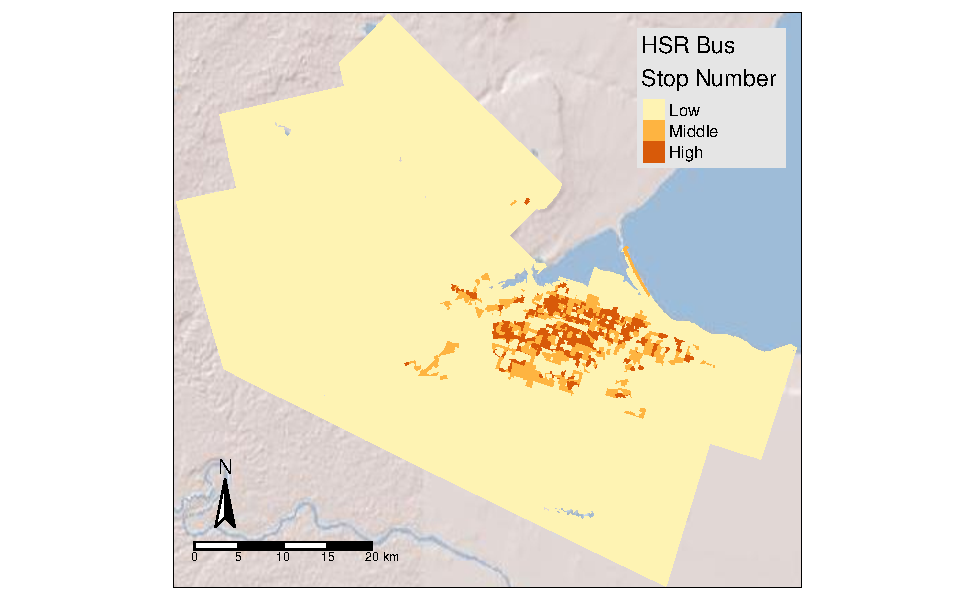
\includegraphics{grocery_store_hamilton_files/figure-latex/unnamed-chunk-10-1.pdf}
\caption{\label{fig::hsr_stops}HSR Bus Stop Number at Dissemination
Areas in Hamilton, Ontario}
\end{figure}

\section{Zero Inflated Negative Binomial Regression
Results}\label{zero-inflated-negative-binomial-regression-results}

Table \ref{tab:regression_results} below shows the regression results.

\begin{table}
\begin{center}
\begin{footnotesize}
\begin{tabular}{l c}
\hline
 & Zero inflated negative binomial model \\
\hline
Count model: Spatial lag of grocery store count                               & $-2.99^{***}$   \\
                                                                              & $(0.84)$        \\
Count model: Percentage of population aged below 24 years old                 & $0.03$          \\
                                                                              & $(0.04)$        \\
Count model: Percentage of population aged above 65 years old                 & $0.02$          \\
                                                                              & $(0.02)$        \\
Count model: Percentage of population don't know official language            & $-0.03$         \\
                                                                              & $(0.10)$        \\
Count model: Percentage of population don't speak official language at home   & $0.17^{**}$     \\
                                                                              & $(0.06)$        \\
Count model: Percentage of population live in single detached houses          & $-0.01^{\cdot}$ \\
                                                                              & $(0.01)$        \\
Count model: Percentage of population have annual total income less than 40K  & $-0.03$         \\
                                                                              & $(0.03)$        \\
Count model: Percentage of population have annual total income more than 100K & $-0.02$         \\
                                                                              & $(0.04)$        \\
Count model: Percentage of population that are married or live in common-law  & $0.03$          \\
                                                                              & $(0.03)$        \\
Count model: Natural log of (population density + 1)                          & $-0.38^{*}$     \\
                                                                              & $(0.17)$        \\
Count model: Natural log of distance from DA centroid to Hamilton downtown    & $-0.50^{**}$    \\
                                                                              & $(0.19)$        \\
Zero model: Spatial lag of grocery store count                                & $-8.62^{*}$     \\
                                                                              & $(3.38)$        \\
Zero model: Percentage of population don't speak official language at home    & $0.14$          \\
                                                                              & $(0.11)$        \\
Zero model: Percentage of population that are married or live in common-law   & $0.11$          \\
                                                                              & $(0.07)$        \\
Zero model: Natural log of (population density + 1)                           & $-1.71^{*}$     \\
                                                                              & $(0.74)$        \\
Zero model: Number of HSR bus stops (50-75 percentile)                        & $-2.73^{***}$   \\
                                                                              & $(0.72)$        \\
Zero model: Number of HSR bus stops (75-100 percentile)                       & $-1.50^{*}$     \\
                                                                              & $(0.74)$        \\
Zero model: Natural log of area size in square kilometres                     & $-2.36^{**}$    \\
                                                                              & $(0.76)$        \\
\hline
AIC                                                                           & $508.91$        \\
Log Likelihood                                                                & $-233.45$       \\
Num. obs.                                                                     & $876$           \\
\hline
\multicolumn{2}{l}{\tiny{$^{***}p<0.001$; $^{**}p<0.01$; $^{*}p<0.05$; $^{\cdot}p<0.1$}}
\end{tabular}
\end{footnotesize}
\caption{Regression results}
\label{tab:regression_results}
\end{center}
\end{table}

\section{Discussion and Conclusion}\label{discussion-and-conclusion}

\renewcommand\refname{References}
\bibliography{mybibfile.bib}


\end{document}
